\section{Sprint 5 : Gestion des stocks, notifications, rapports et tableaux de bord}

\subsection{Introduction}

Après le traitement des interventions préventives et correctives, ce cinquième Sprint est consacré aux fonctions de suivi et de pilotage de la maintenance. Il porte sur la gestion des pièces de rechange et des mouvements de stock, sur le centre de notifications, sur les tableaux de bord ainsi que sur la génération et la programmation des rapports.

{\sloppy
Ces fonctionnalités complètent le processus opérationnel mis en place dans les Sprints précédents. La gestion des stocks assure la disponibilité des pièces nécessaires aux interventions et la traçabilité de leur consommation. Les notifications informent les acteurs des événements qui les concernent. Les tableaux de bord et les rapports fournissent aux responsables une vision synthétique des activités de maintenance.
\par}

Ce chapitre présente les objectifs et le Sprint Backlog, puis la conception du domaine des stocks et du pilotage. Il décrit ensuite les fonctionnalités réalisées et les principaux indicateurs calculés, avant de présenter les tests de validation.

\subsection{Objectifs du Sprint}

L'objectif principal de ce Sprint est de fournir à l'entreprise les moyens de suivre ses ressources techniques et d'évaluer la performance de ses activités de maintenance.

Les objectifs spécifiques sont les suivants :

\begin{itemize}
    \item gérer le catalogue des pièces de rechange ;
    \item suivre les quantités disponibles et réservées ;
    \item enregistrer les mouvements de stock et les ajustements ;
    \item gérer les demandes de pièces et leur cycle de traitement ;
    \item associer les pièces consommées aux ordres de travail ;
    \item conserver les journaux de lubrification ;
    \item diffuser les notifications relatives aux événements de maintenance ;
    \item fournir des tableaux de bord adaptés aux rôles ;
    \item calculer les principaux indicateurs de maintenance ;
    \item générer des rapports aux formats PDF, Excel et CSV ;
    \item programmer l'exécution périodique de certains rapports.
\end{itemize}

À la fin du Sprint, l'administrateur doit pouvoir tenir à jour le catalogue et les quantités, le technicien doit pouvoir demander et consommer des pièces, et chaque acteur doit disposer des notifications, des indicateurs et des rapports correspondant à son rôle.

\subsection{Sprint Backlog}

Le tableau~\ref{tab:sprint5-backlog} recense les tâches planifiées pour ce Sprint.

{\footnotesize
\setlength{\tabcolsep}{4pt}
\begin{longtable}{|p{0.9cm}|>{\raggedright\arraybackslash}p{9.1cm}|>{\raggedright\arraybackslash}p{1.6cm}|>{\raggedright\arraybackslash}p{1.6cm}|}
\caption{Sprint Backlog du Sprint 5}
\label{tab:sprint5-backlog}\\
\hline
\textbf{ID} & \textbf{Tâche} & \textbf{Priorité} & \textbf{Statut} \\
\hline
\endfirsthead

\hline
\textbf{ID} & \textbf{Tâche} & \textbf{Priorité} & \textbf{Statut} \\
\hline
\endhead

S5-01 &
Développer le catalogue des pièces de rechange. &
Haute & Réalisé \\
\hline

S5-02 &
Mettre en place le suivi des quantités disponibles et réservées. &
Haute & Réalisé \\
\hline

S5-03 &
Enregistrer les mouvements de stock et les ajustements. &
Haute & Réalisé \\
\hline

S5-04 &
Gérer les demandes de pièces et leurs états. &
Haute & Réalisé \\
\hline

S5-05 &
Développer les journaux de lubrification. &
Moyenne & Réalisé \\
\hline

S5-06 &
Mettre en place le centre de notifications et les compteurs de lecture. &
Moyenne & Réalisé \\
\hline

S5-07 &
Développer les tableaux de bord adaptés aux rôles. &
Haute & Réalisé \\
\hline

S5-08 &
Calculer les indicateurs de maintenance. &
Haute & Réalisé \\
\hline

S5-09 &
Générer les rapports aux formats PDF, Excel et CSV. &
Haute & Réalisé \\
\hline

S5-10 &
Mettre en place les rapports planifiés. &
Moyenne & Réalisé \\
\hline

S5-11 &
Vérifier les calculs, les exports et les notifications par des tests. &
Haute & Réalisé \\
\hline

\end{longtable}}

User Stories associées :

\begin{itemize}
    \item \textbf{US18 :} en tant qu'administrateur, je souhaite gérer le catalogue et les niveaux de stock afin d'assurer la disponibilité des pièces ;
    \item \textbf{US19 :} en tant que technicien, je souhaite demander des pièces et déclarer leur consommation afin de tracer leur utilisation ;
    \item \textbf{US20 :} en tant qu'utilisateur, je souhaite consulter les notifications qui me concernent afin de suivre les événements importants ;
    \item \textbf{US21 :} en tant qu'utilisateur, je souhaite consulter un tableau de bord adapté à mon rôle afin de suivre l'activité de maintenance ;
    \item \textbf{US22 :} en tant qu'administrateur, je souhaite générer et exporter des rapports afin d'analyser les performances.
\end{itemize}

\subsection{Conception du Sprint}

\subsubsection{Diagramme des cas d'utilisation}

La figure~\ref{fig:usecase-stocks-reporting} présente les cas d'utilisation du domaine des stocks et du pilotage. L'administrateur gère le catalogue, les stocks et les ajustements, les demandes de pièces et les journaux de lubrification ; il consulte les mouvements, le tableau de bord et les notifications, génère et exporte des rapports et peut en programmer. Le technicien traite les demandes de pièces, consulte les mouvements, les notifications, le tableau de bord et les rapports auxquels son rôle donne accès. L'opérateur consulte ses notifications et son tableau de bord. Le planificateur automatique déclenche les rapports programmés, qui s'appuient sur le même mécanisme de génération que les rapports demandés manuellement.

\begin{figure}[H]
    \centering
    \IfFileExists{figures/usecase-stocks-reporting.png}{%
        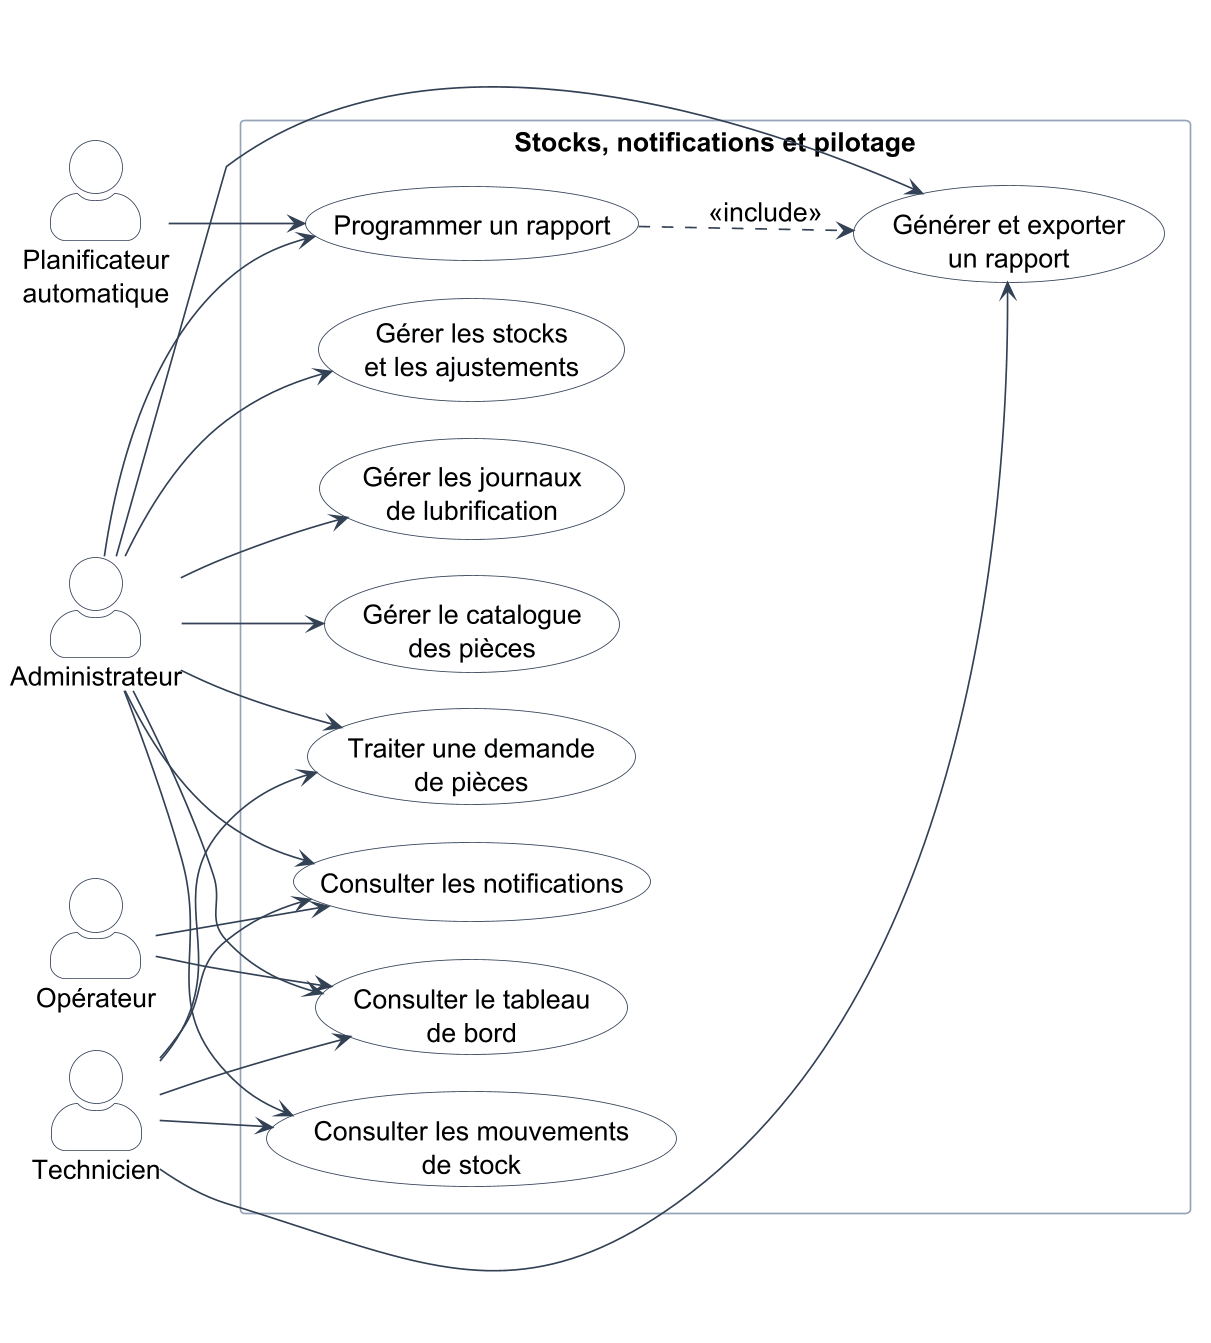
\includegraphics[width=0.92\textwidth,height=0.8\textheight,keepaspectratio]{figures/usecase-stocks-reporting.png}%
    }{%
        \fbox{\parbox[c][7cm][c]{0.92\textwidth}{\centering\itshape Diagramme à insérer\\[2mm]\texttt{figures/usecase-stocks-reporting.png}}}%
    }
    \caption{Diagramme des cas d'utilisation du Sprint 5}
    \label{fig:usecase-stocks-reporting}
\end{figure}

\subsubsection{Diagramme d'activités du traitement d'une demande de pièces}

La figure~\ref{fig:activity-part-request} présente le cycle de traitement d'une demande de pièces. La réservation permet de réserver une quantité sans la retirer immédiatement du stock. La consommation effective n'est enregistrée qu'au moment de l'utilisation de la pièce dans l'intervention.

\begin{figure}[H]
    \centering
    \IfFileExists{figures/activity-part-request.png}{%
        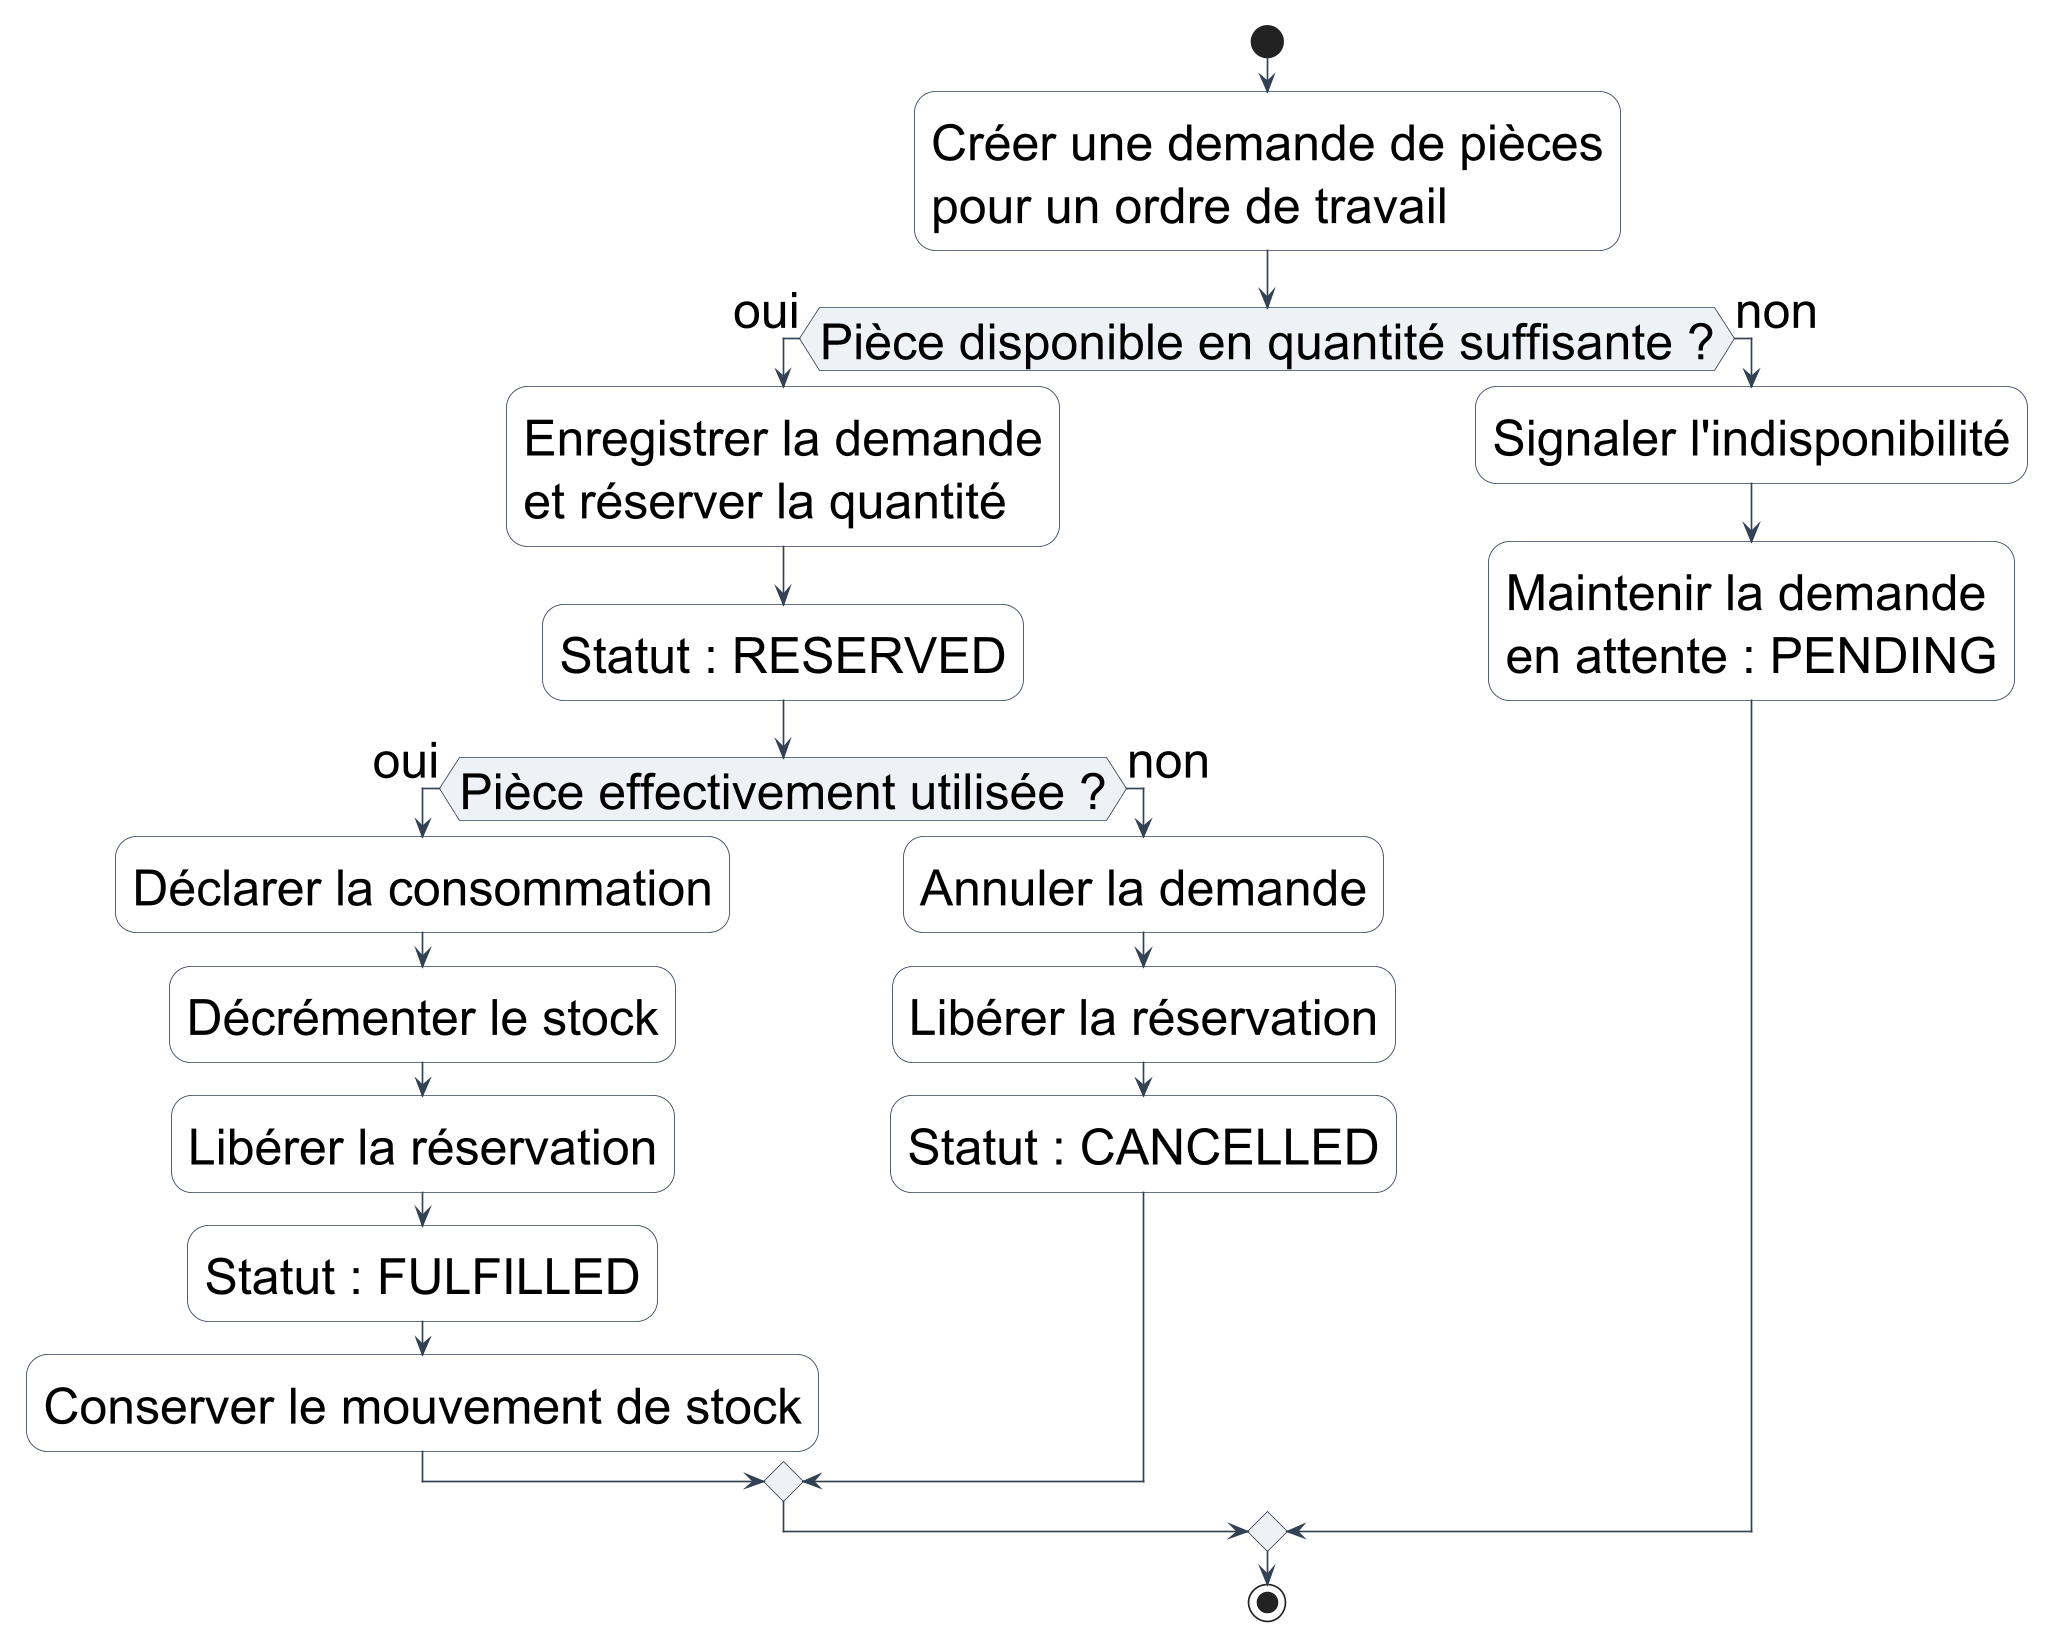
\includegraphics[width=0.8\textwidth,height=0.74\textheight,keepaspectratio]{figures/activity-part-request.png}%
    }{%
        \fbox{\parbox[c][7cm][c]{0.92\textwidth}{\centering\itshape Diagramme à insérer\\[2mm]\texttt{figures/activity-part-request.png}}}%
    }
    \caption{Diagramme d'activités du traitement d'une demande de pièces}
    \label{fig:activity-part-request}
\end{figure}

\subsubsection{Diagramme d'états d'une demande de pièces}

Une demande de pièces ne modifie le stock qu'à partir de l'état réservé. La figure~\ref{fig:state-part-request} présente les états successifs et les transitions autorisées.

À sa création, la demande est à l'état \texttt{PENDING}. Elle ne bloque encore aucune quantité : elle signale seulement un besoin exprimé par le technicien. Si la quantité demandée est disponible, la demande devient \texttt{RESERVED} et la quantité correspondante est retenue sur le stock, sans être physiquement retirée.

Tant que la réservation n'est pas consommée, elle peut être libérée et la demande revient à l'état \texttt{PENDING}, ce qui rend la quantité de nouveau mobilisable pour d'autres interventions. En revanche, dès que la consommation est enregistrée, la demande passe à l'état \texttt{FULFILLED} : cet état est définitif, car le mouvement de stock correspondant est conservé dans le journal.

Une demande peut également être annulée, soit avant toute réservation en cas de refus ou d'abandon, soit après réservation lorsque les pièces ne sont finalement pas utilisées. Dans les deux cas, l'état \texttt{CANCELLED} est terminal et le stock n'est pas impacté.

\begin{figure}[H]
    \centering
    \IfFileExists{figures/state-part-request.png}{%
        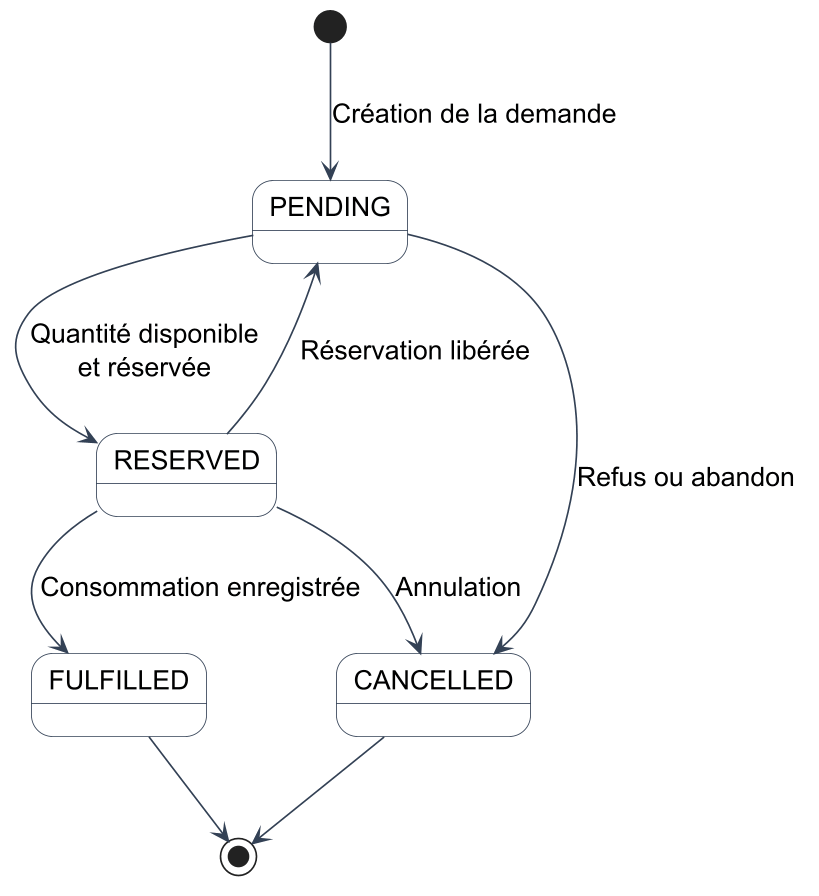
\includegraphics[width=0.72\textwidth,height=0.72\textheight,keepaspectratio]{figures/state-part-request.png}%
    }{%
        \fbox{\parbox[c][7cm][c]{0.92\textwidth}{\centering\itshape Diagramme à insérer\\[2mm]\texttt{figures/state-part-request.png}}}%
    }
    \caption{Diagramme d'états d'une demande de pièces}
    \label{fig:state-part-request}
\end{figure}
\subsubsection{Diagramme de séquence de la génération d'un rapport}

La figure~\ref{fig:sequence-report} présente les échanges entre l'administrateur, l'interface, l'API, le service de calcul des indicateurs, le générateur de documents et la base de données.

La requête est d'abord enregistrée sous la forme d'une ligne à l'état « en attente », ce qui permet à l'interface de rendre la main immédiatement. La collecte des données, la mise en forme et l'écriture du fichier s'exécutent ensuite en arrière-plan. Une fois le document produit, son empreinte est calculée, sa date d'expiration est fixée et une notification est adressée au demandeur. Le même enchaînement est réutilisé par le planificateur pour les rapports récurrents : un rapport programmé ne possède pas de chemin de génération distinct.

\begin{figure}[H]
    \centering
    \IfFileExists{figures/sequence-report.png}{%
        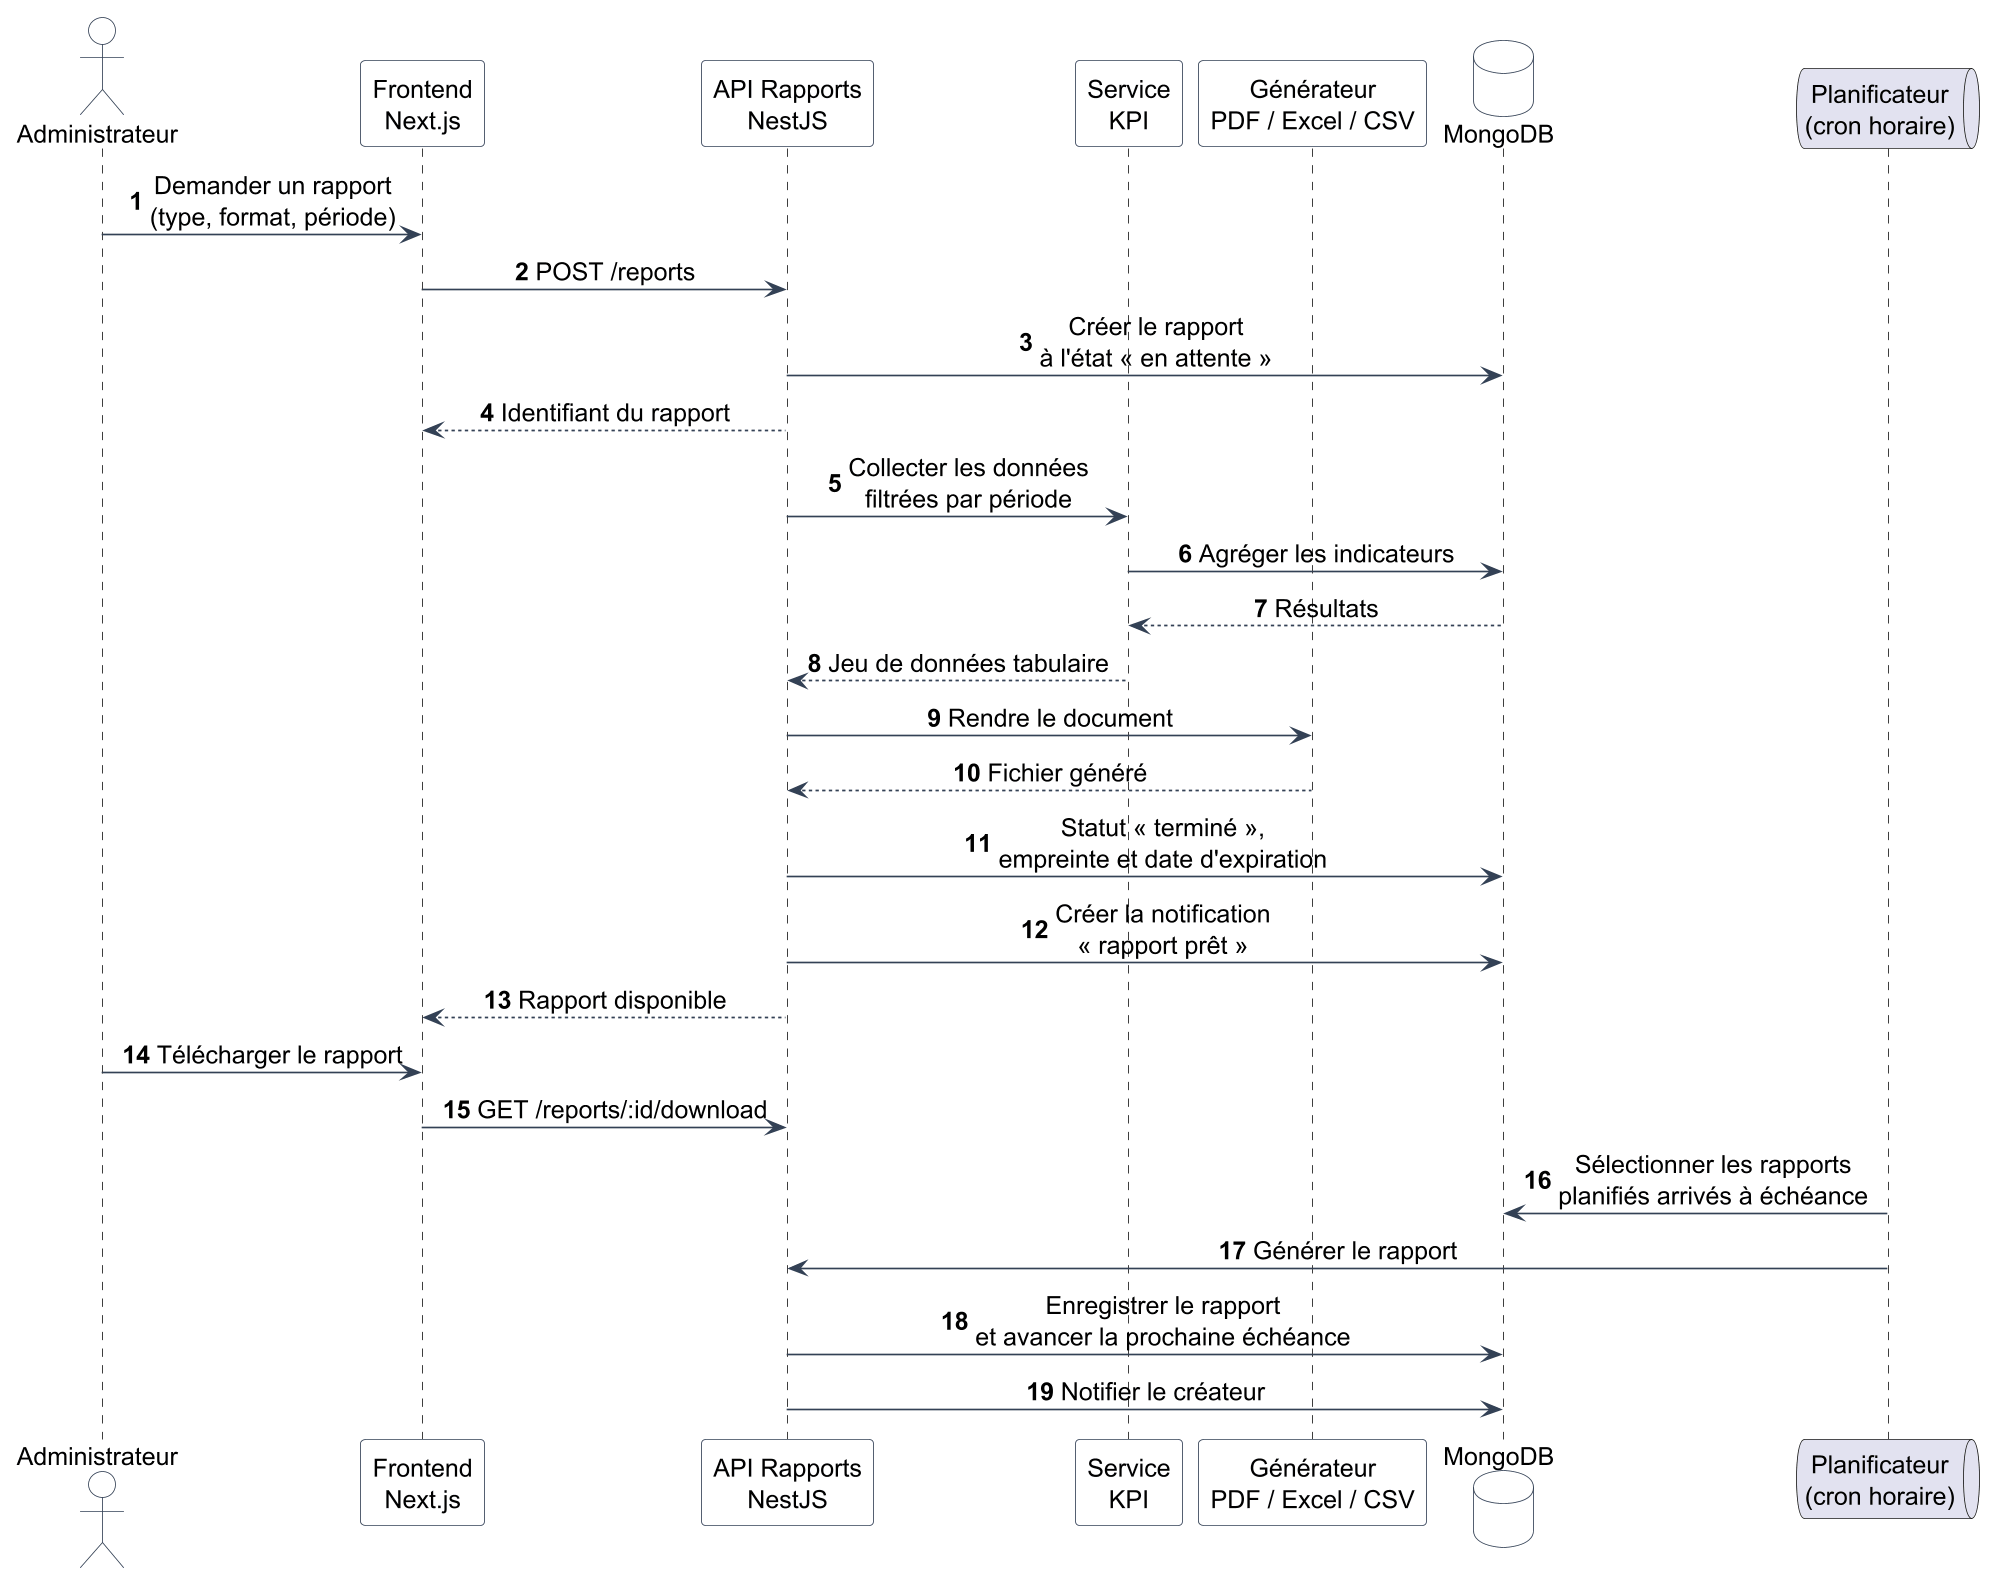
\includegraphics[width=\textwidth,height=0.8\textheight,keepaspectratio]{figures/sequence-report.png}%
    }{%
        \fbox{\parbox[c][7cm][c]{0.92\textwidth}{\centering\itshape Diagramme à insérer\\[2mm]\texttt{figures/sequence-report.png}}}%
    }
    \caption{Diagramme de séquence de la génération d'un rapport}
    \label{fig:sequence-report}
\end{figure}

\subsubsection{Diagramme de séquence de la consommation d'une pièce}

La figure~\ref{fig:sequence-stock-consume} présente la mise à jour du stock lors de la déclaration des pièces utilisées. La quantité réservée est convertie en mouvement de sortie et le stock disponible est recalculé.

Avant tout décompte, l'API vérifie que la demande existe pour cet ordre de travail et que la quantité déclarée reste couverte par la réservation. Si la réservation est suffisante, le stock physique et la quantité réservée sont décrémentés ensemble, puis un mouvement de sortie est consigné avec le rattachement à l'ordre de travail. Le stock affiché est ainsi recalculé à partir des deux compteurs, et non retranché à la volée. Si la quantité déclarée dépasse ce qui était réservé, l'opération est refusée : le technicien doit d'abord obtenir une réservation complémentaire, ce qui évite de consommer une pièce engagée par une autre intervention.

\begin{figure}[H]
    \centering
    \IfFileExists{figures/sequence-stock-consume.png}{%
        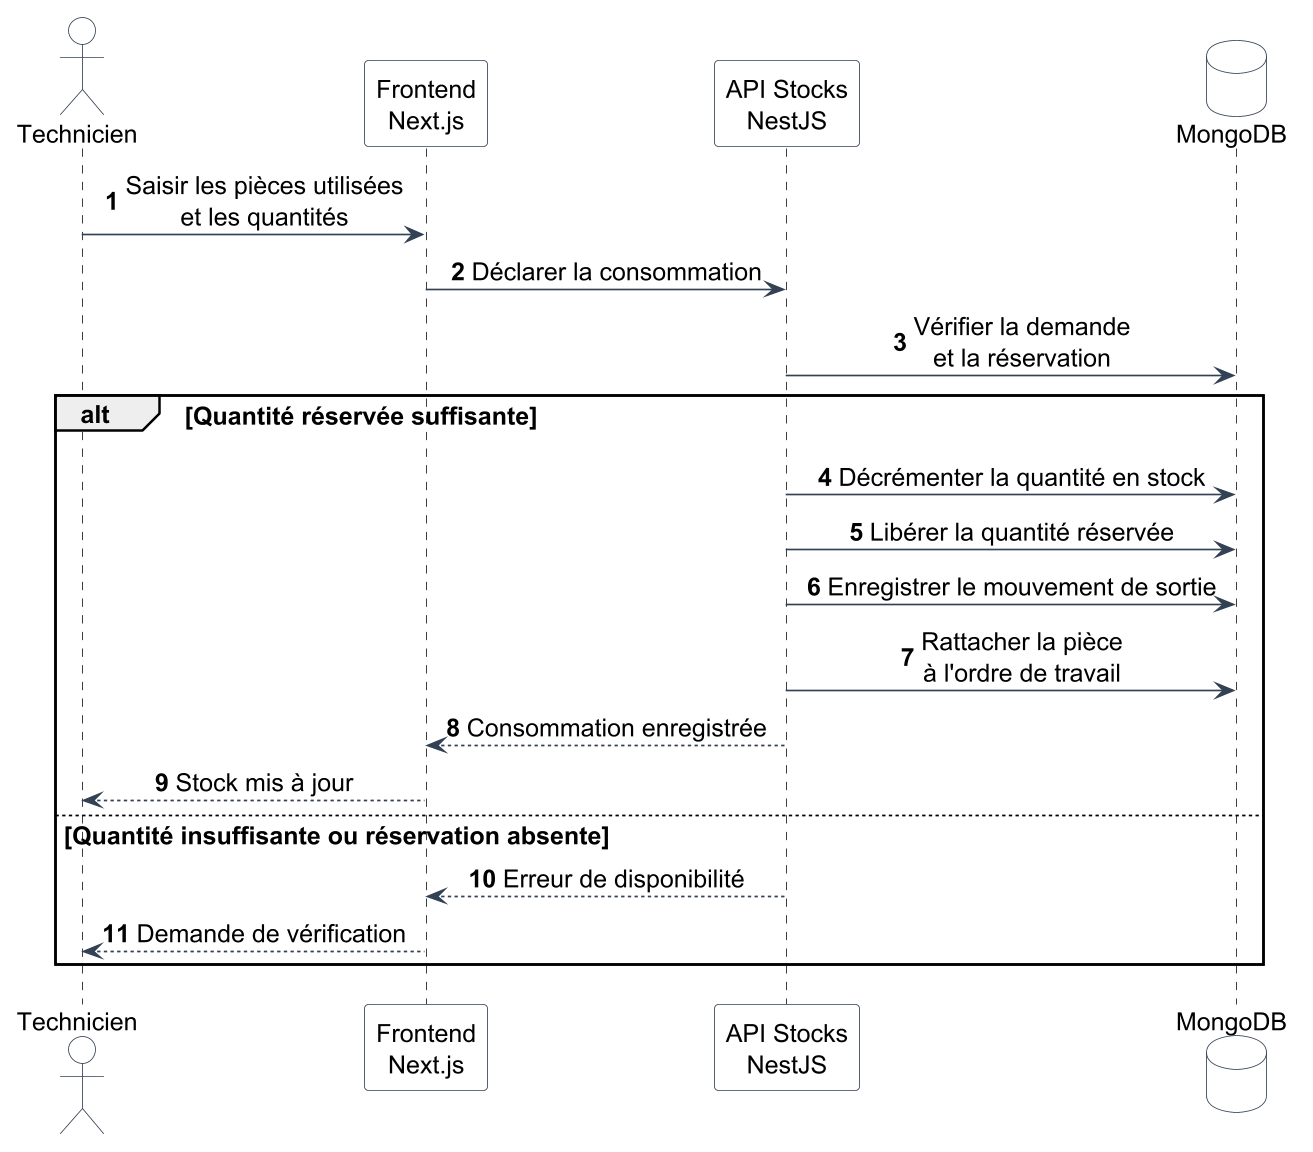
\includegraphics[width=\textwidth,height=0.78\textheight,keepaspectratio]{figures/sequence-stock-consume.png}%
    }{%
        \fbox{\parbox[c][7cm][c]{0.92\textwidth}{\centering\itshape Diagramme à insérer\\[2mm]\texttt{figures/sequence-stock-consume.png}}}%
    }
    \caption{Diagramme de séquence de la consommation d'une pièce}
    \label{fig:sequence-stock-consume}
\end{figure}

\subsubsection{Modèle de données du domaine}

Le tableau~\ref{tab:modele-stocks} présente les principales entités du domaine et leur rôle.

\begin{table}[H]
\centering
\caption{Entités du domaine des stocks et du pilotage}
\label{tab:modele-stocks}
\footnotesize
\setlength{\tabcolsep}{4pt}
\begin{tabularx}{\textwidth}{|>{\raggedright\arraybackslash}p{3.2cm}|>{\raggedright\arraybackslash}X|}
\hline
\textbf{Entité} & \textbf{Rôle dans le domaine} \\
\hline
\texttt{Catalogue} & Référentiel des pièces de rechange et de leurs références constructeur \\
\hline
\texttt{Stock} & Quantités disponibles et réservées pour chaque pièce \\
\hline
\texttt{PartRequest} & Demande de pièces rattachée à un ordre de travail \\
\hline
\texttt{StockMovement} & Historique des entrées, sorties, réservations et ajustements \\
\hline
\texttt{Lubrifiant} & Référentiel des lubrifiants utilisés \\
\hline
\texttt{LubrificationLog} & Journal des opérations de lubrification réalisées \\
\hline
\texttt{Notification} & Événement transmis à un utilisateur \\
\hline
\texttt{KPI} & Indicateurs de maintenance calculés pour une machine \\
\hline
\texttt{ScheduledReport} & Configuration d'un rapport exécuté périodiquement \\
\hline
\end{tabularx}
\end{table}

La quantité réellement disponible est obtenue en soustrayant la quantité réservée de la quantité en stock. Cette distinction évite qu'une même pièce soit promise à deux interventions simultanées.

Les indicateurs sont calculés à partir des ordres de travail et des rapports d'intervention. La collecte et la structuration de ces données s'appuient sur les principes de codification et de traçabilité des événements de maintenance \cite{iso14224}.
\subsection{Réalisation}

\subsubsection{Gestion du catalogue et des stocks}

Le catalogue regroupe les pièces de rechange avec leur désignation, leur référence constructeur et les informations utiles à leur identification. L'administrateur peut ajouter une pièce, modifier ses caractéristiques et consulter les niveaux de stock associés.

Chaque pièce dispose d'une quantité en stock et d'une quantité réservée. La quantité réservée correspond aux demandes acceptées mais dont la consommation n'a pas encore été enregistrée. Cette organisation permet de distinguer la quantité physique de la quantité réellement disponible.

L'administrateur peut ajuster un niveau de stock. Chaque ajustement est enregistré comme un mouvement avec sa date, sa quantité et son motif, afin de conserver un historique exploitable.

La liste des pièces propose une recherche et un filtrage par disponibilité. Les pièces dont la quantité disponible devient faible peuvent être signalées dans les tableaux de bord.

\begin{figure}[H]
    \centering
    \IfFileExists{figures/sprint5-stock-list.png}{%
        \includegraphics[width=0.95\textwidth,height=0.82\textheight,keepaspectratio]{figures/sprint5-stock-list.png}%
    }{%
        \fbox{\parbox[c][7cm][c]{0.92\textwidth}{\centering\itshape Capture d'écran à insérer\\[2mm]\texttt{figures/sprint5-stock-list.png}}}%
    }
    \caption{Suivi des pièces de rechange et des niveaux de stock}
    \label{fig:sprint5-stock-list}
\end{figure}

\subsubsection{Demandes de pièces et mouvements}

Une demande de pièces est créée depuis un ordre de travail. Elle précise la pièce concernée, la quantité demandée et l'intervention associée.

Selon la disponibilité, la demande peut être réservée, maintenue en attente ou annulée. La réservation ne modifie pas immédiatement la quantité physique, mais réduit la quantité disponible pour les autres demandes.

Lors de la consommation, le stock est décrémenté et la réservation est libérée. Un mouvement de sortie est enregistré avec le lien vers l'ordre de travail. Cette association permet de reconstituer les pièces utilisées pour une intervention et d'alimenter les analyses de coût.

Les mouvements de stock sont consultables avec leur type, leur quantité, leur date et leur origine. Ce journal constitue la base de la traçabilité des entrées et des sorties de pièces.

\subsubsection{Journaux de lubrification}

La plateforme permet de gérer les lubrifiants utilisés ainsi que les journaux des opérations de lubrification. Une entrée de journal précise la machine ou le module concerné, le lubrifiant utilisé, la date de l'opération et les observations éventuelles.

Ce suivi complète les listes de contrôle préventives, dont certaines tâches prévoient explicitement une lubrification ou un graissage. Il permet de conserver un historique des produits appliqués sur chaque équipement.

\subsubsection{Centre de notifications}

Le centre de notifications regroupe les événements destinés à l'utilisateur connecté. Les notifications peuvent concerner l'affectation d'un ordre de travail, la validation ou le rejet d'une intervention, une demande de pièces, une rupture de stock ou une anomalie détectée.

Chaque notification comporte un type, un contenu, une date et éventuellement une référence vers la machine ou l'ordre de travail concerné. Un compteur indique le nombre de notifications non lues.

L'utilisateur peut marquer une notification comme lue ou la supprimer. Les notifications peuvent également être transmises par courriel lorsque le service de messagerie est configuré. L'envoi par courriel reste optionnel et ne bloque pas le fonctionnement du centre de notifications.

\subsubsection{Tableaux de bord et indicateurs}

Les tableaux de bord présentent une vue synthétique adaptée au rôle de l'utilisateur. L'administrateur dispose d'une vision globale du parc et des interventions. Le technicien consulte ses ordres de travail, ses interventions en cours et son historique. L'opérateur retrouve ses machines, ses opérations préventives et ses notifications.

Les indicateurs sont calculés à partir des ordres de travail et des rapports d'intervention. Les principaux indicateurs utilisés sont le temps moyen entre deux pannes, le temps moyen de réparation et le taux de disponibilité.

Le temps moyen entre deux pannes est calculé par la relation suivante :

\begin{equation}
\mathrm{MTBF} = \frac{\text{Temps total de fonctionnement}}{\text{Nombre de pannes}}
\label{eq:mtbf}
\end{equation}

Le temps moyen de réparation est calculé par :

\begin{equation}
\mathrm{MTTR} = \frac{\text{Temps total de réparation}}{\text{Nombre d'interventions}}
\label{eq:mttr}
\end{equation}

Le taux de disponibilité est obtenu à partir de ces deux indicateurs :

\begin{equation}
\mathrm{D} = \frac{\mathrm{MTBF}}{\mathrm{MTBF} + \mathrm{MTTR}} \times 100
\label{eq:disponibilite}
\end{equation}

Ces indicateurs sont calculés par machine et agrégés pour la flotte d'équipements. Leur définition et leur interprétation suivent les recommandations relatives aux indicateurs de maintenance \cite{en15341}.

Les graphiques sont générés à partir des données de la plateforme et affichés dans les tableaux de bord. Ils permettent de suivre l'évolution des interventions, la répartition des pannes et l'état des stocks.

\begin{figure}[H]
    \centering
    \IfFileExists{figures/sprint5-dashboard.png}{%
        \includegraphics[width=0.95\textwidth,height=0.82\textheight,keepaspectratio]{figures/sprint5-dashboard.png}%
    }{%
        \fbox{\parbox[c][7cm][c]{0.92\textwidth}{\centering\itshape Capture d'écran à insérer\\[2mm]\texttt{figures/sprint5-dashboard.png}}}%
    }
    \caption{Tableau de bord et indicateurs de maintenance}
    \label{fig:sprint5-dashboard}
\end{figure}

\subsubsection{Génération et exportation des rapports}

La plateforme permet de générer des rapports portant sur les machines, les interventions, les ordres de travail, les stocks ou les indicateurs de maintenance. Le tableau~\ref{tab:types-rapports} présente les principaux types de rapports et les formats disponibles.

{\footnotesize
\setlength{\tabcolsep}{4pt}
\begin{table}[H]
\centering
\caption{Types de rapports et formats d'exportation}
\label{tab:types-rapports}
\begin{tabularx}{\textwidth}{|>{\raggedright\arraybackslash}p{4.2cm}|>{\raggedright\arraybackslash}X|>{\raggedright\arraybackslash}p{2.9cm}|}
\hline
\textbf{Type de rapport} & \textbf{Contenu principal} & \textbf{Formats} \\
\hline
Rapport des interventions & Historique, durées, techniciens et pièces utilisées & PDF, Excel, CSV \\
\hline
Rapport des ordres de travail & États, priorités, affectations et délais & PDF, Excel, CSV \\
\hline
Rapport des équipements & Fiche, historique et indicateurs par machine & PDF, Excel, CSV \\
\hline
Rapport des stocks & Quantités disponibles, réservées et mouvements & PDF, Excel, CSV \\
\hline
Rapport des indicateurs & MTBF, MTTR et disponibilité par machine & PDF, Excel, CSV \\
\hline
\end{tabularx}
\end{table}}

Les rapports PDF sont destinés à la consultation et à l'archivage. Les exports Excel et CSV facilitent les traitements complémentaires et l'analyse des données.

L'accès aux rapports est limité selon le rôle et le périmètre de l'utilisateur. Un technicien consulte les rapports relatifs à ses interventions, tandis que l'administrateur dispose d'une vue globale.

\subsubsection{Rapports planifiés}

Certains rapports peuvent être exécutés périodiquement. La configuration précise le type de rapport, la fréquence et les destinataires.

Le planificateur déclenche la génération selon la périodicité définie et conserve la trace de chaque exécution. En cas d'échec, l'erreur est journalisée afin de permettre son diagnostic.

Cette fonctionnalité réduit les manipulations répétitives et facilite le suivi régulier des activités de maintenance.

\subsection{Tests et validation}

Le tableau~\ref{tab:tests-sprint5} présente une synthèse des scénarios vérifiés pour ce Sprint.

{\footnotesize
\setlength{\tabcolsep}{4pt}
\begin{longtable}{|p{0.9cm}|>{\raggedright\arraybackslash}p{7cm}|>{\raggedright\arraybackslash}p{4.7cm}|}
\caption{Scénarios de test du Sprint 5}
\label{tab:tests-sprint5}\\
\hline
\textbf{ID} & \textbf{Scénario} & \textbf{Résultat attendu} \\
\hline
\endfirsthead

\hline
\textbf{ID} & \textbf{Scénario} & \textbf{Résultat attendu} \\
\hline
\endhead

T5-01 &
Création d'une pièce dans le catalogue &
Pièce enregistrée et disponible pour les demandes \\
\hline

T5-02 &
Ajustement du stock d'une pièce &
Mouvement enregistré et quantité mise à jour \\
\hline

T5-03 &
Demande d'une pièce disponible &
Demande réservée et quantité disponible réduite \\
\hline

T5-04 &
Demande d'une pièce en quantité insuffisante &
Demande maintenue en attente \\
\hline

T5-05 &
Consommation d'une pièce réservée &
Stock décrémenté, réservation libérée et mouvement conservé \\
\hline

T5-06 &
Annulation d'une demande réservée &
Réservation libérée et stock disponible rétabli \\
\hline

T5-07 &
Enregistrement d'un journal de lubrification &
Opération conservée avec la machine, le lubrifiant et la date \\
\hline

T5-08 &
Consultation du compteur de notifications &
Nombre de notifications non lues correct \\
\hline

T5-09 &
Marquage d'une notification comme lue &
Compteur mis à jour \\
\hline

T5-10 &
Consultation du tableau de bord par un technicien &
Indicateurs limités à son périmètre \\
\hline

T5-11 &
Calcul du MTTR à partir des interventions &
Valeur cohérente avec les durées enregistrées \\
\hline

T5-12 &
Génération d'un rapport PDF &
Fichier généré et téléchargeable \\
\hline

T5-13 &
Export d'un rapport au format Excel &
Fichier valide et données cohérentes \\
\hline

T5-14 &
Exécution d'un rapport planifié &
Rapport généré à la périodicité définie \\
\hline

\end{longtable}}

Les tests ont confirmé la cohérence entre les demandes de pièces, les réservations et les mouvements de stock. Les calculs d'indicateurs ont été vérifiés à partir de jeux de données de référence, et les exports ont été contrôlés pour les trois formats.

\subsection{Revue du Sprint et conclusion}
\enlargethispage{2\baselineskip}

Lors de la revue, le catalogue des pièces, les mouvements de stock, le centre de notifications, les tableaux de bord et les rapports ont été présentés.

Les principaux résultats du Sprint sont les suivants :

\begin{itemize}
    \item centralisation du catalogue des pièces et des niveaux de stock ;
    \item distinction entre quantité physique, quantité réservée et quantité disponible ;
    \item traçabilité des demandes, des réservations et des consommations ;
    \item conservation des journaux de lubrification ;
    \item diffusion des notifications liées aux événements de maintenance ;
    \item mise à disposition de tableaux de bord adaptés aux rôles ;
    \item calcul des indicateurs MTBF, MTTR et disponibilité ;
    \item génération de rapports PDF, Excel et CSV ;
    \item exécution périodique des rapports planifiés.
\end{itemize}

La rétrospective a souligné l'intérêt de regrouper ces fonctions dans un même Sprint : elles exploitent les données produites par les Sprints précédents et fournissent aux responsables une vision consolidée des activités de maintenance.

Le Sprint 6 sera consacré à la surveillance des équipements connectés et à la maintenance prédictive.